\documentclass[aspectratio=169]{beamer}

\usetheme{metropolis}           % Use metropolis theme
\usepackage[utf8]{inputenc}
\usepackage{graphicx}
\usepackage{eso-pic}
\usepackage{graphics}
\usepackage{tikz}
\usepackage[export]{adjustbox}
\usepackage{multicol}
\usepackage{listings}
\usepackage{helvet}
\usepackage{booktabs}
\usepackage{threeparttable}
\usepackage{marvosym}
\usepackage{hyperref}
\usepackage{xcolor}
\usepackage{soul}	% For strike-through
\usepackage{tcolorbox} % For color box

\newcounter{exercises}

\title{Data Processing in Python\\Using Pandas}
\date{}
\author{DIME Analytics \newline Presented by Luis Eduardo San Martin} % Name of author(s) of session here
\institute{Development Impact Evaluation (DIME) \newline The World Bank }
\setbeamercolor{background canvas}{bg=white}	% Sets background color

% The below command places the World Bank logo and DIME logo to the right corner
\titlegraphic{%
	\begin{picture}(0,0)
	\put(330,-180){\makebox(0,0)[rt]{
\includegraphics[width=3cm]{img/WB_logo}}}
	\end{picture}%
	\begin{picture}(0,0)
	\put(390,-180){\makebox(0,0)[rt]{
\includegraphics[width=1.5cm]{img/i2i}}}
	\end{picture}%
}

%%% Section page with picture of Light bulb
\makeatletter
\defbeamertemplate*{section page}{mytheme}[1][]{
	\centering
	\begin{minipage}{22em}
		\raggedright
		\usebeamercolor[fg]{section title}
		\usebeamerfont{section title}
		\par
		\ifx\insertsubsectionhead\@empty\else%
		\usebeamercolor[fg]{subsection title}%
		\usebeamerfont{subsection title}%
		\fi
		\ifstrempty{#1}{}{%
			\includegraphics[width=100mm, height=60mm]{#1}%
		}
		\\
		\insertsectionhead\\[-1ex]
		\insertsubsectionhead
		\usebeamertemplate*{progress bar in section page}
		
	\end{minipage}
	\par
	\vspace{\baselineskip}
}
\makeatother

%%% Define a command to include picture in section, 
%%% make section, and revert to old template
\newcommand{\sectionpic}[2]{
	\setbeamertemplate{section page}[mytheme][#2]
	\section{#1}
	\setbeamertemplate{section page}[mytheme]
}

%%% The command below allows for the text that contains Stata code
\lstset{ %
	backgroundcolor=\color{white},
	basicstyle=\tiny,
	breakatwhitespace=false,
	breaklines=true,
	captionpos=b,
	commentstyle=\color{green},
	escapeinside={\%*}{*)},
	extendedchars=true,
	frame=single,
	numbers=left,
	numbersep=5pt,
	numberstyle=\tiny\color{gray},
	rulecolor=\color{black},
	showspaces=false,
	showstringspaces=false,
	showtabs=false,
	stringstyle=\color{mauve},
	tabsize=2,
	title=\lstname,
	morekeywords={not,\},\{,preconditions,effects },
	deletekeywords={time}
}

%% The below command creates the ligh bulb logos in the top right corner of the 
\begin{document}
	
	
	%%%%%%%%%%%%%%%%%%%%%%%%%%%%%%%%%%%%%%%%%%% Title slide
	{
		\usebackgroundtemplate{
\includegraphics[height=55mm,right]{img/top_right_corner.pdf}} 
		\maketitle
	}

\begin{frame}

	\frametitle{Overview} % Table of contents slide, comment this block out to remove it
	\tableofcontents % Throughout your presentation, if you choose to use \section{} and \subsection{} commands, these will automatically be printed on this slide as an overview of your presentation

\end{frame}

%%%%%%%%%%%%%%%%%%%%%%%%%%%%%%%%%%%%%%%%%%% Section title slide
\sectionpic{Introduction}{img/section_slide}

%%%%%%%%%%%%%%%%%%%%%%%%%%%%%%%%%%%%%%%%%%% Slide
\begin{frame}{Introduction}

	\begin{itemize}
		\item This session will introduce you to Pandas, the most popular data frames processing library in Python
		\item We'll review:
		\begin{itemize}
			\item Pandas dataframes
			\item Data processing operations
		\end{itemize}
		\item We'll take advantage of your Stata knowledge to establish comparisons between Stata's and Pandas' commands
	\end{itemize}

\end{frame}

%%%%%%%%%%%%%%%%%%%%%%%%%%%%%%%%%%%%%%%%%%% Slide
\begin{frame}{Introduction - Why Pandas if I already know Stata?}

	\begin{itemize}
		\item \textbf{Big data:} though Pandas is not suitable for big data,  the most popular Python big data tools expect you to know it
		\item \textbf{ML:} If you ever want to implement a ML pipeline using Python, you'll need Pandas for your data transformation
		\item \textbf{Cloud platforms:} Cloud platforms assume Python much more often than Stata, and Pandas is the library assumed for data processing
		\item \textbf{General Python data work:} Being the go-to library for data processing, most Python data work libraries assume Pandas knowledge -- for example: many of them use Pandas dataframes or series objects as inputs
	\end{itemize}

\end{frame}

%%%%%%%%%%%%%%%%%%%%%%%%%%%%%%%%%%%%%%%%%%% Section title slide
\sectionpic{Getting Started}{img/section_slide}

%%%%%%%%%%%%%%%%%%%%%%%%%%%%%%%%%%%%%%%%%%% Slide
\begin{frame}{Getting started}

	\begin{itemize}
		\item We'll use \href{http://colab.research.google.com}{Google Colab} today
		\item It is similar to a Google Doc but for coding, and runs Python by default
	\end{itemize}

\end{frame}

%%%%%%%%%%%%%%%%%%%%%%%%%%%%%%%%%%%%%%%%%%% Slide
\begin{frame}{Getting started}

	\begin{itemize}
		\item Go to https://colab.research.google.com
		\item Click on \texttt{NEW NOTEBOOK} if you're already logged in, or go to \texttt{File > New notebook} if you're not
	\end{itemize}

	\begin{multicols}{2}

		\begin{figure}
			\centering
			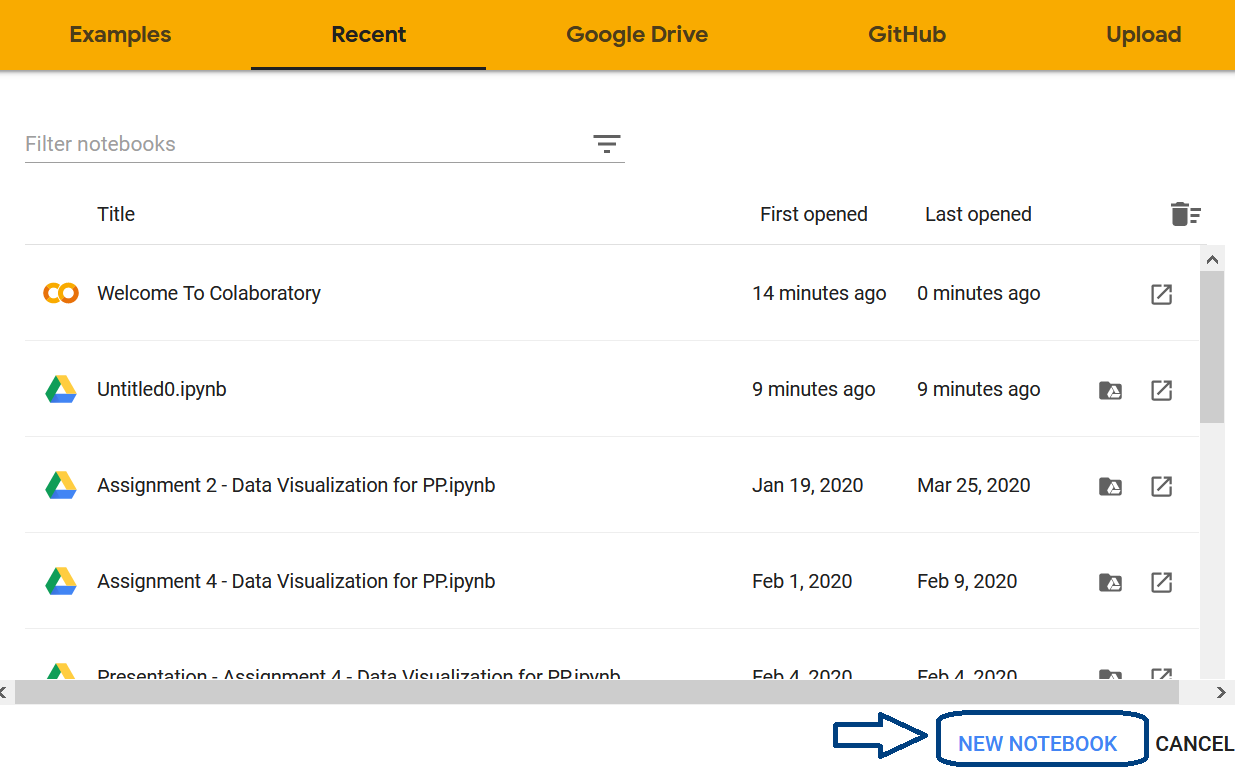
\includegraphics[width=0.9\linewidth]{img/new_nb_logged_in.png}
			\caption{Do this if you're already logged in}
		\end{figure}
		\begin{figure}
			\centering
			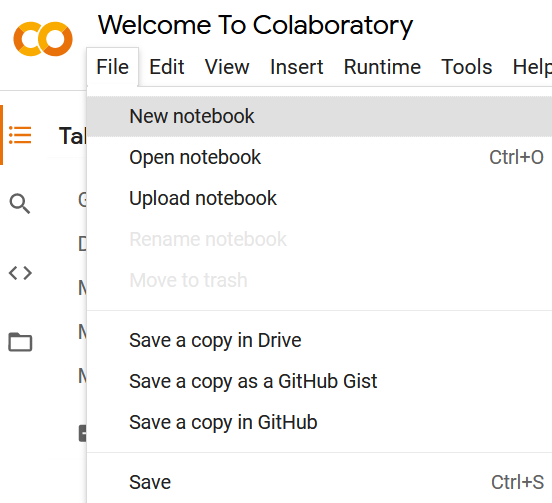
\includegraphics[width=0.6\linewidth]{img/new_nb_not_logged_in.png}
			\caption{Do this if you're not -- you'll be prompted to log in}
		\end{figure}

	\end{multicols}

\end{frame}

%%%%%%%%%%%%%%%%%%%%%%%%%%%%%%%%%%%%%%%%%%% Section title slide
\sectionpic{The Pandas library}{img/section_slide}

%%%%%%%%%%%%%%%%%%%%%%%%%%%%%%%%%%%%%%%%%%% Slide
\begin{frame}{Pandas}

	\begin{itemize}
		\item Pandas is used for data processing and data analysis
		\item Use the following command to import Pandas to your notebook:
	\end{itemize}

	\hspace{7mm} \texttt{\textcolor{purple}{import} pandas as \textcolor{purple}{pd}}

\end{frame}

%%%%%%%%%%%%%%%%%%%%%%%%%%%%%%%%%%%%%%%%%%% Subsection
\subsection{Pandas dataframes}

%%%%%%%%%%%%%%%%%%%%%%%%%%%%%%%%%%%%%%%%%%% Slide
\begin{frame}{Pandas}

	\textbf{Dataframes}

	\begin{multicols}{2}
	
		\begin{itemize}
			\item A dataframe is a two-dimensional data structure
			\item They are very often used to work with data structures where every row represents a unit of observation and every column represents an observation's attribute
			\item The Stata equivalent to dataframes are datasets
		\end{itemize}
		\begin{figure}
			\centering
			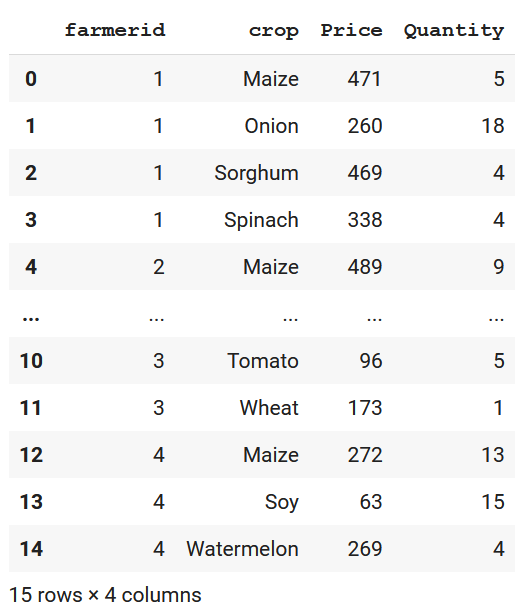
\includegraphics[width=0.8\linewidth]{img/dataframe.png}
		\end{figure}

	\end{multicols}

\end{frame}

%%%%%%%%%%%%%%%%%%%%%%%%%%%%%%%%%%%%%%%%%%% Slide
\begin{frame}{Pandas}

	\textbf{Dataframes}

	There are several ways to create a dataframe from scratch. One of the easiest is:

	\begin{enumerate}
		\item Define a list of strings with the column names
		\begin{figure}
			
\includegraphics[width=0.8\linewidth]{img/column_names.png}
		\end{figure}
		\item Define a list for \textbf{each observation}
		\begin{figure}
			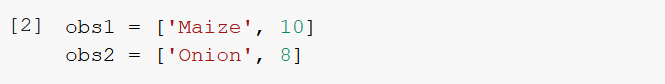
\includegraphics[width=0.8\linewidth]{img/observation_lists.png}
		\end{figure}
		\item Wrap all of the observation lists in another list
		\begin{figure}
			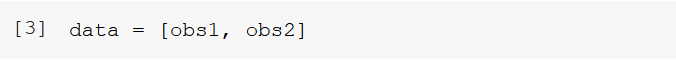
\includegraphics[width=0.8\linewidth]{img/data_list.png}
		\end{figure}

	\end{enumerate}

\end{frame}

%%%%%%%%%%%%%%%%%%%%%%%%%%%%%%%%%%%%%%%%%%% Slide
\begin{frame}{Pandas}

	\textbf{Dataframes}

	\begin{enumerate}
		\setcounter{enumi}{3}
		\item Use the lists \texttt{data} and \texttt{column\_names} as inputs in the \texttt{DataFrame()} command
		\begin{figure}
			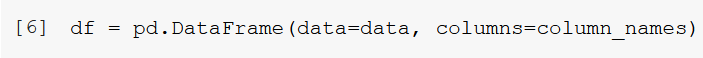
\includegraphics[width=0.8\linewidth]{img/dataframe_definition.png}
		\end{figure}
		\item Now your dataframe is defined in the variable \texttt{df}. You can use that name to refer to it or print it, as in:
		\begin{figure}
			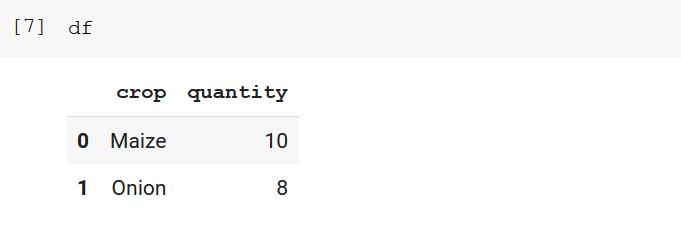
\includegraphics[width=0.8\linewidth]{img/df.png}
		\end{figure}
	\end{enumerate}

\end{frame}

%%%%%%%%%%%%%%%%%%%%%%%%%%%%%%%%%%%%%%%%%%% Slide
\begin{frame}{Pandas}

	\textbf{Dataframes}

	Another way to create a dataframe from zero is to define an empty dataframe and then create its columns individually.
	\begin{figure}
		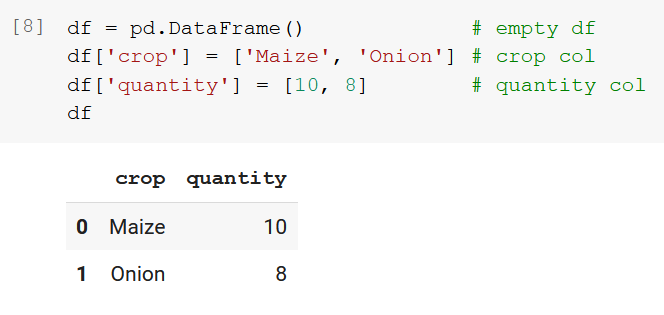
\includegraphics[width=0.8\linewidth]{img/df_definition2.png}
	\end{figure}

\end{frame}

%%%%%%%%%%%%%%%%%%%%%%%%%%%%%%%%%%%%%%%%%%% Slide
\begin{frame}{Pandas}

	\textbf{Dataframes}

	\begin{itemize}
		\item Every row and column of a dataframe has a \textbf{label}
		\item Row labels are represented by the index
		\item Column labels are represented by the column names
	\end{itemize}
	\begin{figure}
		\centering
		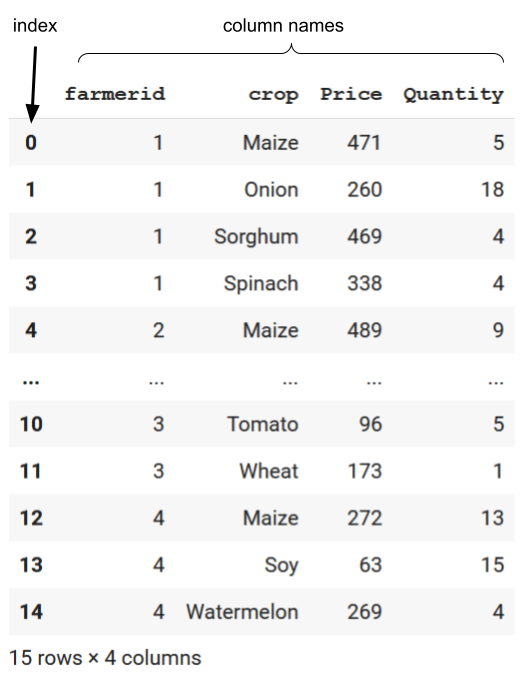
\includegraphics[width=0.43\linewidth]{img/dataframe_indices.png}
	\end{figure}

\end{frame}

%%%%%%%%%%%%%%%%%%%%%%%%%%%%%%%%%%%%%%%%%%% Section title slide
\sectionpic{Data processing}{img/section_slide}

%%%%%%%%%%%%%%%%%%%%%%%%%%%%%%%%%%%%%%%%%%% Subsection
\subsection{Reading data}

%%%%%%%%%%%%%%%%%%%%%%%%%%%%%%%%%%%%%%%%%%% Slide
\begin{frame}{Data processing}

	\textbf{Reading data}

	\begin{itemize}
		\item In our work, we'll seldom need to define a dataframe from scratch
		\item More often, we'll load a pre-existing data file with Pandas
		\item To load a \texttt{.csv} file into a dataframe, we use the command \texttt{read_csv()}
	\end{itemize}

\end{frame}

%%%%%%%%%%%%%%%%%%%%%%%%%%%%%%%%%%%%%%%%%%% Slide
\begin{frame}{}

\end{frame}

\end{document}
